\documentclass[border=2mm]{standalone}

\usepackage{fontspec}
\usepackage{unicode-math}

\usepackage{pgfplots}
\pgfplotsset{compat=1.18}
\usetikzlibrary{arrows.meta, 
  calc, 
  positioning, 
  decorations.pathreplacing, 
  calligraphy}

\usepackage{xcolor}
\definecolor{den-1}{HTML}{111111}   % Đen #111111
\definecolor{den-2}{HTML}{222222}   % Đen #222222
\definecolor{den-3}{HTML}{333333}   % Đen #333333
\definecolor{den-4}{HTML}{444444}   % Đen #444444
\definecolor{den-5}{HTML}{555555}   % Đen #555555
\definecolor{den-6}{HTML}{666666}   % Đen #666666

% Thiết lập vị trí đặt nhãn gốc tọa độ
\tikzset{
  >=Stealth,
  originlabel/.style={
    font=\small\sf,
    anchor=north east, % Vị trí tương đối so với gốc
    yshift=-0.1ex,     % Điều chỉnh vị trí dọc một chút
    xshift=-0.1ex      % Điều chỉnh vị trí ngang một chút
  }
}

\begin{document}

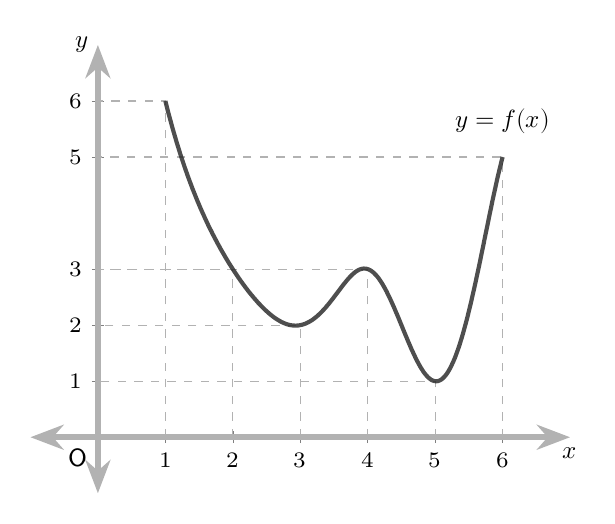
\begin{tikzpicture}

\begin{axis}[
    font=\small\sf,
    axis lines=middle,
    axis line style={<->, line width=2pt, color=den-6!50},
    xlabel=$x$, ylabel=$y$,
    xlabel style={below, font=\small\sf},
    ylabel style={left, font=\small\sf},
    xmin=-1, xmax=7,
    ymin=-1, ymax=7,
    xtick={1,2,3,4,5,6},
    ytick={1,2,3,5,6},
    tick label style={font=\footnotesize\sf},
    clip=false,
]

\node[originlabel] at (axis cs:0,0) {O};

\draw [dashed, color=den-6!50] (1,0) -- (1,6) -- (0,6);
\draw [dashed, color=den-6!50] (2,0) -- (2,3) -- (0,3);
\draw [dashed, color=den-6!50] (3,0) -- (3,2) -- (0,2);
\draw [dashed, color=den-6!50] (4,0) -- (4,3) -- (0,3);
\draw [dashed, color=den-6!50] (5,0) -- (5,1) -- (0,1);
\draw [dashed, color=den-6!50] (6,0) -- (6,5) -- (0,5);

\node at (6,5) [anchor=south, yshift=5] {$y=f(x)$};


\addplot[smooth, line width=1.5pt, color=den-2, opacity=.8] coordinates {
  (1.000, 6.000)
  (1.017, 5.920)
  (1.033, 5.842)
  (1.050, 5.765)
  (1.067, 5.690)
  (1.084, 5.616)
  (1.100, 5.543)
  (1.117, 5.472)
  (1.134, 5.402)
  (1.151, 5.333)
  (1.167, 5.266)
  (1.184, 5.200)
  (1.201, 5.135)
  (1.217, 5.071)
  (1.234, 5.009)
  (1.251, 4.947)
  (1.268, 4.887)
  (1.284, 4.828)
  (1.301, 4.769)
  (1.318, 4.712)
  (1.334, 4.656)
  (1.351, 4.601)
  (1.368, 4.546)
  (1.385, 4.493)
  (1.401, 4.440)
  (1.418, 4.389)
  (1.435, 4.338)
  (1.452, 4.288)
  (1.468, 4.239)
  (1.485, 4.190)
  (1.502, 4.143)
  (1.518, 4.096)
  (1.535, 4.050)
  (1.552, 4.004)
  (1.569, 3.960)
  (1.585, 3.916)
  (1.602, 3.872)
  (1.619, 3.829)
  (1.635, 3.787)
  (1.652, 3.746)
  (1.669, 3.705)
  (1.686, 3.665)
  (1.702, 3.625)
  (1.719, 3.586)
  (1.736, 3.547)
  (1.753, 3.509)
  (1.769, 3.471)
  (1.786, 3.434)
  (1.803, 3.398)
  (1.819, 3.361)
  (1.836, 3.326)
  (1.853, 3.291)
  (1.870, 3.256)
  (1.886, 3.222)
  (1.903, 3.188)
  (1.920, 3.154)
  (1.936, 3.121)
  (1.953, 3.089)
  (1.970, 3.057)
  (1.987, 3.025)
  (2.003, 2.994)
  (2.020, 2.963)
  (2.037, 2.932)
  (2.054, 2.902)
  (2.070, 2.873)
  (2.087, 2.843)
  (2.104, 2.814)
  (2.120, 2.786)
  (2.137, 2.758)
  (2.154, 2.730)
  (2.171, 2.703)
  (2.187, 2.676)
  (2.204, 2.649)
  (2.221, 2.623)
  (2.237, 2.597)
  (2.254, 2.572)
  (2.271, 2.547)
  (2.288, 2.523)
  (2.304, 2.499)
  (2.321, 2.475)
  (2.338, 2.452)
  (2.355, 2.429)
  (2.371, 2.406)
  (2.388, 2.385)
  (2.405, 2.363)
  (2.421, 2.342)
  (2.438, 2.322)
  (2.455, 2.302)
  (2.472, 2.282)
  (2.488, 2.263)
  (2.505, 2.245)
  (2.522, 2.227)
  (2.538, 2.209)
  (2.555, 2.192)
  (2.572, 2.176)
  (2.589, 2.160)
  (2.605, 2.145)
  (2.622, 2.130)
  (2.639, 2.116)
  (2.656, 2.103)
  (2.672, 2.091)
  (2.689, 2.079)
  (2.706, 2.067)
  (2.722, 2.057)
  (2.739, 2.047)
  (2.756, 2.038)
  (2.773, 2.030)
  (2.789, 2.022)
  (2.806, 2.015)
  (2.823, 2.009)
  (2.839, 2.004)
  (2.856, 2.000)
  (2.873, 1.997)
  (2.890, 1.994)
  (2.906, 1.993)
  (2.923, 1.992)
  (2.940, 1.992)
  (2.957, 1.993)
  (2.973, 1.995)
  (2.990, 1.998)
  (3.007, 2.002)
  (3.023, 2.006)
  (3.040, 2.012)
  (3.057, 2.019)
  (3.074, 2.026)
  (3.090, 2.035)
  (3.107, 2.044)
  (3.124, 2.054)
  (3.140, 2.065)
  (3.157, 2.077)
  (3.174, 2.090)
  (3.191, 2.104)
  (3.207, 2.119)
  (3.224, 2.135)
  (3.241, 2.151)
  (3.258, 2.169)
  (3.274, 2.187)
  (3.291, 2.206)
  (3.308, 2.226)
  (3.324, 2.246)
  (3.341, 2.268)
  (3.358, 2.290)
  (3.375, 2.312)
  (3.391, 2.336)
  (3.408, 2.360)
  (3.425, 2.384)
  (3.441, 2.409)
  (3.458, 2.435)
  (3.475, 2.461)
  (3.492, 2.487)
  (3.508, 2.513)
  (3.525, 2.540)
  (3.542, 2.567)
  (3.559, 2.594)
  (3.575, 2.620)
  (3.592, 2.647)
  (3.609, 2.674)
  (3.625, 2.700)
  (3.642, 2.726)
  (3.659, 2.751)
  (3.676, 2.776)
  (3.692, 2.800)
  (3.709, 2.824)
  (3.726, 2.846)
  (3.742, 2.868)
  (3.759, 2.888)
  (3.776, 2.907)
  (3.793, 2.925)
  (3.809, 2.942)
  (3.826, 2.956)
  (3.843, 2.970)
  (3.860, 2.981)
  (3.876, 2.991)
  (3.893, 2.998)
  (3.910, 3.004)
  (3.926, 3.008)
  (3.943, 3.010)
  (3.960, 3.009)
  (3.977, 3.007)
  (3.993, 3.002)
  (4.010, 2.996)
  (4.027, 2.987)
  (4.043, 2.976)
  (4.060, 2.962)
  (4.077, 2.947)
  (4.094, 2.929)
  (4.110, 2.909)
  (4.127, 2.888)
  (4.144, 2.864)
  (4.161, 2.838)
  (4.177, 2.810)
  (4.194, 2.780)
  (4.211, 2.748)
  (4.227, 2.715)
  (4.244, 2.680)
  (4.261, 2.643)
  (4.278, 2.605)
  (4.294, 2.565)
  (4.311, 2.524)
  (4.328, 2.482)
  (4.344, 2.439)
  (4.361, 2.394)
  (4.378, 2.349)
  (4.395, 2.303)
  (4.411, 2.256)
  (4.428, 2.209)
  (4.445, 2.161)
  (4.462, 2.112)
  (4.478, 2.064)
  (4.495, 2.015)
  (4.512, 1.966)
  (4.528, 1.917)
  (4.545, 1.868)
  (4.562, 1.819)
  (4.579, 1.771)
  (4.595, 1.723)
  (4.612, 1.676)
  (4.629, 1.629)
  (4.645, 1.583)
  (4.662, 1.539)
  (4.679, 1.495)
  (4.696, 1.452)
  (4.712, 1.410)
  (4.729, 1.370)
  (4.746, 1.331)
  (4.763, 1.294)
  (4.779, 1.259)
  (4.796, 1.225)
  (4.813, 1.194)
  (4.829, 1.164)
  (4.846, 1.137)
  (4.863, 1.112)
  (4.880, 1.089)
  (4.896, 1.068)
  (4.913, 1.051)
  (4.930, 1.035)
  (4.946, 1.022)
  (4.963, 1.012)
  (4.980, 1.005)
  (4.997, 1.001)
  (5.013, 0.999)
  (5.030, 1.000)
  (5.047, 1.004)
  (5.064, 1.012)
  (5.080, 1.022)
  (5.097, 1.035)
  (5.114, 1.051)
  (5.130, 1.071)
  (5.147, 1.093)
  (5.164, 1.119)
  (5.181, 1.147)
  (5.197, 1.179)
  (5.214, 1.214)
  (5.231, 1.252)
  (5.247, 1.293)
  (5.264, 1.337)
  (5.281, 1.383)
  (5.298, 1.433)
  (5.314, 1.486)
  (5.331, 1.542)
  (5.348, 1.600)
  (5.365, 1.661)
  (5.381, 1.725)
  (5.398, 1.791)
  (5.415, 1.861)
  (5.431, 1.932)
  (5.448, 2.006)
  (5.465, 2.082)
  (5.482, 2.161)
  (5.498, 2.242)
  (5.515, 2.325)
  (5.532, 2.409)
  (5.548, 2.496)
  (5.565, 2.584)
  (5.582, 2.674)
  (5.599, 2.766)
  (5.615, 2.858)
  (5.632, 2.952)
  (5.649, 3.047)
  (5.666, 3.144)
  (5.682, 3.240)
  (5.699, 3.338)
  (5.716, 3.436)
  (5.732, 3.534)
  (5.749, 3.633)
  (5.766, 3.731)
  (5.783, 3.829)
  (5.799, 3.927)
  (5.816, 4.025)
  (5.833, 4.121)
  (5.849, 4.217)
  (5.866, 4.311)
  (5.883, 4.404)
  (5.900, 4.496)
  (5.916, 4.586)
  (5.933, 4.674)
  (5.950, 4.759)
  (5.967, 4.842)
  (5.983, 4.923)
  (6.000, 5.000)
};


\end{axis}

\end{tikzpicture}

\end{document}